\documentclass[a4paper,12pt]{article}

%%% Работа с русским языком
\usepackage{cmap}					% поиск в PDF
\usepackage{mathtext} 				% русские буквы в фомулах
\usepackage[T2A]{fontenc}			% кодировка
\usepackage[utf8]{inputenc}			% кодировка исходного текста
\usepackage[english,russian]{babel}	% локализация и переносы

%\usepackage{biblatex} %Imports biblatex package

\usepackage{subcaption}
\usepackage{graphicx}
\usepackage{makecell}
\usepackage{hyperref}
\usepackage[dvipsnames]{xcolor}
\usepackage{bbm}

%%% Дополнительная работа с математикой
\usepackage{amsfonts,amssymb,amsthm,mathtools} % AMS
\usepackage{amsmath}
\usepackage{icomma} % "Умная" запятая: $0,2$ --- число, $0, 2$ --- перечисление
\usepackage{amsthm}

%% Номера формул
%\mathtoolsset{showonlyrefs=true} % Показывать номера только у тех формул, на которые есть \eqref{} в тексте.

%% Шрифты
\usepackage{euscript}	 % Шрифт Евклид
\usepackage{mathrsfs} % Красивый матшрифт

%% Свои команды
\DeclareMathOperator{\sgn}{\mathop{sgn}}

%% Перенос знаков в формулах (по Львовскому)
\newcommand*{\hm}[1]{#1\nobreak\discretionary{}
	{\hbox{$\mathsurround=0pt #1$}}{}}

%%% Работа с картинками
\usepackage{graphicx}  % Для вставки рисунков
\graphicspath{{images/}{images2/}}  % папки с картинками
\setlength\fboxsep{3pt} % Отступ рамки \fbox{} от рисунка
\setlength\fboxrule{1pt} % Толщина линий рамки \fbox{}
\usepackage{wrapfig} % Обтекание рисунков и таблиц текстом
\usepackage{caption}
\captionsetup{labelsep=period} %. вместо : в рис

%%% Работа с таблицами
\usepackage{array,tabularx,tabulary,booktabs} % Дополнительная работа с таблицами
\usepackage{longtable}  % Длинные таблицы
\usepackage{multirow} % Слияние строк в таблице

\usepackage{extsizes} % Возможность сделать 14-й шрифт
\usepackage{geometry} % Простой способ задавать поля
\geometry{top=25mm}
\geometry{bottom=35mm}
\geometry{left=10mm}
\geometry{right=15mm}

\renewcommand{\leq}{\leqslant}
\renewcommand{\geq}{\geqslant}
\renewcommand{\top}{\mathsf{T}}

\newcommand{\tr}{\text{tr}}
%\newcommand{\det}{\text{det}}

\begin{document}
	\section{Выпуклые множества}
	
	\begin{enumerate}
		\item $f(x) = \max\limits_{i=\overline{1,p}}(a_i x + b_i )$, где $x,\;a_i,\;b_i\in \mathbb{R}$
		
		По определению сопряженная функция вводится следующим образом: 
		$$
		f^*(y) = \sup\limits_x~\left[xy - f(x)\right] = \sup\limits_x~\left[xy - \max\limits_{i=\overline{1,p}} (a_i x + b_i)\right].
		$$
		$f(x)$ --- поточечный максимум линейных функций, поэтому эта функция кусочно-линейная и является выпуклой. Найдем точки <<переключения>> между линейными функциями. Без ограничения общности предположим, что $a_i \leq a_{i+1},\; i=\overline{1,p-1}$, всегда можно переупорядочить функции таким образом. Для определенности предположим также, что каждая из $p$ линейных функций $a_i x + b_i$ в каких-то точках равна $f(x)$, то есть является максимумом, в противном случае уберем такие функции из рассмотрения.
		
		Используя описанные предположения, найдем точки <<переключения>> между линейными функциями в $f(x)$, а именно точки <<переключения>> между $i$ и $i+1$ линейной функцией $\tilde{x}_i,\; i=\overline{1,p-1}$:
		$$
		a_i \tilde{x}_i + b_i = a_{i+1} \tilde{x}_i + b_{i+1};\quad \tilde{x}_i = \frac{b_i - b_{i+1}}{a_{i+1} - a_i}. 
		$$
		Из определения $f^*(y)$ можно видеть, что сопряженная функция будет ограничена только при $y\in[a_1;a_p]$, при этом максимум будет достигаться в точках <<переключения>> $\tilde{x}_i$ между функциями. Это можно понять, расписав  $f^*(y)$ через индикаторные функции $\mathbbm{1}$:
		\begin{equation*}
		\begin{aligned}
		f^*(y) = \sup\limits_x \Biggr[x &\left(y - a_1 \mathbbm{1}(x \leq \tilde{x}_1) - a_p \mathbbm{1}(\tilde{x}_{p-1} < x) - \sum\limits_{i=2}^{p-1} a_i \mathbbm{1}(\tilde{x}_{i-1} < x \leq \tilde{x}_i)\right) - \\		
		& b_1 \mathbbm{1}(x \leq \tilde{x}_1)  - b_p \mathbbm{1}(\tilde{x}_{p-1} < x) - \sum\limits_{i=2}^{p-1} b_i \mathbbm{1}(\tilde{x}_{i-1} < x \leq \tilde{x}_i)\Biggr].
		\end{aligned}
		\end{equation*}
		Действительно, для $y\in[a_1;a_p]$ максимум достигается в точках $\tilde{x}_i$, $y$ вне этого интервала приводят к ненулевому линейному коэффициенту при $x$, поэтому функция будет неограничена сверху. Также этот факт виден из геометрической интерпретации сопряженной функции. Тогда общая формула $f^*(y)$ записывается в виде:
		$$
		f^*(y) = 
		\begin{cases}
			\dfrac{ b_i - b_{i+1}}{a_{i+1}-a_i} (y - a_i) - b_i,\quad y\in[a_i;a_{i+1}],\; i=\overline{1,p-1} \\
			\infty,\quad \text{else}.
		\end{cases}
		$$
		Из итоговой формулы можно видеть, что сопряженная функция на своей области определения $\text{dom}(f^*) = [a_1;a_p]$ также является кусочно-линейной.
		
		\item $g(\mathbf{x}) = \inf_{\mathbf{x}_1+...+\mathbf{x}_k = \mathbf{x}}(f_1(\mathbf{x}_1) + ... + f_k(\mathbf{x}_k))$, где $f_i$ --- выпуклые функции.
		
		Распишем $g^*(\mathbf{x})$ по определению:
		
		$$
			g^*(\mathbf{y}) =  \sup\limits_{\mathbf{x}}~\left[\mathbf{x}^\mathsf{T}\mathbf{y} - g(\mathbf{x})\right] = \sup\limits_{\substack{\mathbf{x_1},...,\mathbf{x_k},\\ \mathbf{x}_1+...+\mathbf{x}_k = \mathbf{x}}}~\left[\left(\sum\limits_{i=1}^k \mathbf{x_i}^\mathsf{T}\right)\mathbf{y} - \inf_{\mathbf{x}_1+...+\mathbf{x}_k = \mathbf{x}}(f_1(\mathbf{x}_1) + ... + f_k(\mathbf{x}_k))\right].
		$$
		Заметим, что $\inf\limits_\mathbf{x}(h(\mathbf{x})) = -\sup\limits_\mathbf{x}(-h(\mathbf{x}))$. Поэтому можно переписать формулу в более простой форме:
		$$
		g^*(\mathbf{y}) =  \sup\limits_{\mathbf{x}_1,...,\mathbf{x}_k}~\left[\sum\limits_{i=1}^k \mathbf{x_i}^\mathsf{T} \mathbf{y} - \sum\limits_{i=1}^k f_i(\mathbf{x_i})\right] = \sum\limits_{i=1}^k f_i^*(\mathbf{x}_i),
		$$
		здесь было использовано определение сопряженных к $f_i$ функций. Таким образом, сопряженная функция к инфимальной свертке функций --- это сумма сопряженных функций.
		
		\item 
		
		$f(\mathbf{X}) = \text{tr}(\mathbf{X}^{-1}),\; \text{dom}(f) = \mathbf{S}^n_{++} $.
		
		Запишем определение сопряженной функции:
		$$
		f^*(\mathbf{Y}) = \sup\limits_{\mathbf{x}}~\left[\text{tr}(\mathbf{X}^\mathsf{T}\mathbf{Y}) - \text{tr}(\mathbf{X}^{-1}) \right].
		$$
		
		Найдем область определения сопряженной функции. Докажем, что $\text{dom}(f^*) = -\mathbf{S}^n_{+}$. Запишем разложение $\mathbf{Y}$ по собственным векторам и приведем к диагональному виду $\mathbf{X}$ в базисе из собственных векторов $\mathbf{Y}$: 
		$$
		\mathbf{Y} = \mathbf{Q} \mathbf{\Lambda} \mathbf{Q}^\mathsf{T} = \sum\limits_{i=1}^n \lambda_i \mathbf{q}_i \mathbf{q}_i^\mathsf{T};\quad
		 \mathbf{X} =\mathbf{Q} \mathbf{A} \mathbf{Q}^\mathsf{T} = \sum\limits_{i=1}^n \alpha_i \mathbf{q}_i \mathbf{q}_i^\mathsf{T},\; \alpha_i > 0. 
		$$
		В этом случае под супремумом находится следующая функция:
		$$
		\text{tr}(\mathbf{X}^\mathsf{T}\mathbf{Y}) - \text{tr}(\mathbf{X}^{-1}) = \text{tr}(\mathbf{\Lambda} \mathbf{A} - \mathbf{A}^{-1}) = \sum_{i=1}^n \lambda_i \alpha_i - \sum_{i=1}^n 1/\alpha_i.
		$$
		Из формулы можно видеть, что если хотя бы для одного $i$ выполнено $\lambda_i > 0$ (то есть в спектре $\mathbf{Y}$ есть положительное собственное значение), то данная функция неограничена сверху, поэтому областью определения сопряженной функции является $\mathbf{Y} \in -\mathbf{S}^n_{+}$, 
		
		В номере 3.1(f) первого задания было доказано, что $\text{tr}(\mathbf{X}^{-1})$ является выпуклой функцией на $\mathbf{S}^n_{++}$. Кроме того, $\text{tr}(\mathbf{X}^\mathsf{T}\mathbf{Y})$ --- аффинная по $\mathbf{X}$ как линейная функция. Таким образом, $\text{tr}(\mathbf{X}^\mathsf{T}\mathbf{Y}) - \text{tr}(\mathbf{X}^{-1})$ является вогнутой функцией.
		
		Найдем супремум функции аналитически. Из вогнутости и дифференцируемости функции следует, что можно найти ее максимум, приравняв градиент функции нулю:
		$$
		\frac{\partial (\text{tr}(\mathbf{X}^\mathsf{T}\mathbf{Y}) - \text{tr}(\mathbf{X}^{-1}))}{\partial \mathbf{X}} = \mathbf{Y} + \mathbf{X}^{-2} = \mathbf{0},\quad \mathbf{X} = (-\mathbf{Y})^{-1/2}.
		$$
 		Таким образом, сопряженная функция имеет вид:
 		$$
 		f^*(\mathbf{Y}) = -2~ \text{tr}((-\mathbf{Y})^{1/2}).
 		$$
		
	\end{enumerate}
	
	\section{Условия оптимальности}
	\begin{enumerate}
		\item Требуется решить следующую задачу:
		\begin{equation*}
		\begin{aligned}
			& \min\limits_\mathbf{x}\; \mathbf{c}^\mathsf{T} \mathbf{x} \\
			\text{s.t.}\; & \mathbf{x}^\mathsf{T} \mathbf{A} \mathbf{x} \leq 1,
		\end{aligned}
		\end{equation*}
		где $\mathbf{A}\in\mathbf{S}^n_{++}$.
	
	Так как $\mathbf{A}\in\mathbf{S}^n_{++}$, сделаем замену $\mathbf{z} = \mathbf{A}^{1/2}\mathbf{x}$ и обозначим $\mathbf{d} = - \mathbf{A}^{-1/2} \mathbf{c}$. Получаем эквивалентную задачу максимизации линейной функции на единичном шаре:
	\begin{equation*}
		\begin{aligned}
			& \max\limits_\mathbf{z}\; \mathbf{d}^\mathsf{T} \mathbf{z} \\
			\text{s.t.}\; & \Vert\mathbf{z}\Vert^2_2 \leq 1.
		\end{aligned}
	\end{equation*}
	Данная задача является выпуклой и для нее можно было бы использовать условия ККТ, но получим решение $\mathbf{z}^*$ более простым способом, используя неравенство КБШ:
	$$
	\mathbf{d}^\mathsf{T} \mathbf{z} \leq \Vert\mathbf{d}\Vert_2 \Vert\mathbf{z}\Vert_2 \leq \Vert\mathbf{d}\Vert_2,\quad \mathbf{d}^\mathsf{T}\mathbf{z}^* = \Vert\mathbf{d}\Vert_2,\quad \mathbf{z}^* = \mathbf{d} / \Vert\mathbf{d}\Vert_2.
	$$
	Таким образом, после обратной замены координат, получаем точку минимума исходной задачи $\mathbf{x}^*$ и значение целевой функции $\mathbf{c}^\mathsf{T} \mathbf{x}^*$ в ней:
	$$
	\mathbf{x}^* =  \frac{-1}{\Vert \mathbf{A}^{-1/2} \mathbf{c}\Vert_2} \mathbf{A}^{-1}\mathbf{c} = \frac{-1}{\sqrt{\mathbf{c}^\mathsf{T} \mathbf{A}^{-1} \mathbf{c}}} \mathbf{A}^{-1}\mathbf{c};\quad \mathbf{c}^\mathsf{T} \mathbf{x}^* = - \sqrt{\mathbf{c}^\mathsf{T} \mathbf{A}^{-1} \mathbf{c}}.
	$$
	
	\item Требуется решить следующую оптимизационную задачу: 
	\begin{equation*}
		\begin{aligned}
			& \min\limits_{\mathbf{X}\in\mathbf{S}_{++}^n}\; \tr(\mathbf{X}) - \log(\det(\mathbf{X})) \\
			\text{s.t.}\; & \mathbf{X}\mathbf{z} = \mathbf{y},
		\end{aligned}
	\end{equation*}
	где $\mathbf{y},\mathbf{z}\in\mathbb{R}^n$ и $\mathbf{y}^\mathsf{T}\mathbf{z} = 1$.
	
	Данная задача выпуклая. Действительно, целевая функция является суммой аффинной функции (след) и вогнутой функции (на лекции было доказана выпуклость логарифма определителя матрицы, здесь перед ним стоит минус). Функциональные ограничения в задача линейные и область определения является выпуклым множеством ($\mathbf{S}_{++}^n$).  Запишем функцию Лагранжа для данной задачи:
	$$
	L(\mathbf{X}, \lambda) = \tr(\mathbf{X}) - \log(\det(\mathbf{X})) + \lambda^\top (\mathbf{X}\mathbf{z} - \mathbf{y}),\; \lambda \in \mathbb{R}^n
	$$ 
	Выпишем условия ККТ:
	\begin{equation*}
	\begin{aligned}
		&\frac{\partial L(\mathbf{X}, \lambda)}{\partial \mathbf{X}} = \mathbf{0};\\
		&\mathbf{X}\mathbf{z} = \mathbf{y};\\
		&\mathbf{X} \succ 0.
	\end{aligned}
	\end{equation*}
	Найдем градиенты  каждого из слагаемых в функции Лагранжа:
	\begin{equation*}
	\begin{aligned}
	&\frac{\partial}{\partial \mathbf{X}} \log(\det(\mathbf{X})) = 
	\frac{1}{\det\mathbf{X}} \frac{\partial \det{(\mathbf{X}})}{\partial \mathbf{X}} = \frac{1}{\det\mathbf{X}} \text{adj}(\mathbf{X})^\top = \mathbf{X}^{-\top}\\
	&\frac{\partial}{\partial \mathbf{X}}  (\lambda^\top (\mathbf{X}\mathbf{z} - \mathbf{y})) = \frac{1}{2} (\lambda \mathbf{z}^\top + \mathbf{z}\lambda^\top)\\
	&\frac{\partial}{\partial \mathbf{X}} \tr{(\mathbf{X}}) = \mathbf{I}.
	\end{aligned}
	\end{equation*}
	Таким образом, условия на стационарную точку функции Лагранжа переписывается в виде:
	$$
	\frac{\partial L(\mathbf{X}, \lambda)}{\partial \mathbf{X}} = \mathbf{I} - \mathbf{X}^{-\top} + \frac{1}{2} (\lambda \mathbf{z}^\top + \mathbf{z}\lambda^\top) = \mathbf{0};\quad \mathbf{X}^{-1} = \mathbf{I} + \frac{1}{2} (\lambda \mathbf{z}^\top + \mathbf{z}\lambda^\top).
	$$
	Из ограничения равенства можно выразить $\mathbf{z} = \mathbf{X}^{-1}\mathbf{y}$. Используем это выражение, домножив формулу $\mathbf{X}^{-1}$ справа на $\mathbf{y}$. Также учтем условия равенства единице скалярного произведения векторов $\mathbf{z}$ и $\mathbf{y}$, домножив после этого полученное равенство слева на $\mathbf{y}^\top$: 
	$$
	\mathbf{z} = \mathbf{y} + \frac{1}{2}\lambda +\frac{1}{2} \mathbf{z}\lambda^\top\mathbf{y};\quad  1 = \mathbf{y}^\top \mathbf{z} = \Vert \mathbf{y} \Vert_2^2 + \lambda^\top \mathbf{y};\quad \lambda^\top \mathbf{y} =  1 - \Vert \mathbf{y} \Vert_2^2.
	$$
	Подставим формулу для $\lambda^\top \mathbf{y}$ в исходное равенство на $\mathbf{z}$ и выразим из него множитель Лагранжа $\lambda$:
	$$
	\mathbf{z} = \mathbf{y} + \frac{1}{2}\lambda + \frac{1}{2}(1 - \Vert \mathbf{y} \Vert_2^2) \mathbf{z};\quad \lambda = -2\mathbf{y} + (1 + \Vert \mathbf{y} \Vert_2^2) \mathbf{z}.
	$$ 
	Таким образом, подставив $\lambda$ в выражение на $\mathbf{X}^{-1}$, получаем явный вид обратной матрицы предполагаемого решения задачи:
	$$
	\mathbf{X}^{-1} = \mathbf{I} + \frac{1}{2}\left(  1 +  \Vert \mathbf{y} \Vert_2^2\right) \mathbf{z}\mathbf{z}^\top - \mathbf{y}\mathbf{z}^\top - \mathbf{z}\mathbf{y}^\top.
	$$
	Теперь требуется найти исходную матрицу $\mathbf{X}$. Догадаемся до решения $\tilde{\mathbf{X}}$ и докажем, что оно действительно является $\mathbf{X}$ проверкой $\mathbf{X} \mathbf{X}^{-1} = \mathbf{I}$.
	\begin{equation*}\begin{aligned}
	&\tilde{\mathbf{X}} = \mathbf{I} + \mathbf{y} \mathbf{y}^\top - \frac{1}{\Vert\mathbf{z}\Vert_2^2} \mathbf{z} \mathbf{z}^\top; \\
	\tilde{\mathbf{X}} \mathbf{X}^{-1} &= \left(\mathbf{I} + \mathbf{y} \mathbf{y}^\top - \frac{1}{\Vert\mathbf{z}\Vert_2^2} \mathbf{z} \mathbf{z}^\top\right) 
	\left(\mathbf{I} + \frac{1}{2}\left(  1 +  \Vert \mathbf{y} \Vert_2^2\right) \mathbf{z}\mathbf{z}^\top - \mathbf{y}\mathbf{z}^\top - \mathbf{z}\mathbf{y}^\top\right) \\
	&=\mathbf{I} + \frac{1}{2}\left(  1 +  \Vert \mathbf{y} \Vert_2^2\right) \mathbf{z}\mathbf{z}^\top - \mathbf{y}\mathbf{z}^\top - \mathbf{z}\mathbf{y}^\top + \\
	 &\quad\;\mathbf{y} \mathbf{y}^\top + \frac{1}{2}\left(  1 +  \Vert \mathbf{y} \Vert_2^2\right) \mathbf{y} \mathbf{y}^\top \mathbf{z}\mathbf{z}^\top - \mathbf{y} \mathbf{y}^\top\mathbf{y}\mathbf{z}^\top - \mathbf{y} \mathbf{y}^\top\mathbf{z}\mathbf{y}^\top - \\
	 &\quad\;\frac{1}{\Vert\mathbf{z}\Vert_2^2} \mathbf{z} \mathbf{z}^\top - \frac{1}{2}\left(  1 +  \Vert \mathbf{y} \Vert_2^2\right) \frac{1}{\Vert\mathbf{z}\Vert_2^2} \mathbf{z} \mathbf{z}^\top \mathbf{z}\mathbf{z}^\top + \frac{1}{\Vert\mathbf{z}\Vert_2^2} \mathbf{z} \mathbf{z}^\top \mathbf{y}\mathbf{z}^\top + \frac{1}{\Vert\mathbf{z}\Vert_2^2} \mathbf{z} \mathbf{z}^\top \mathbf{z}\mathbf{y}^\top \\
	 &=\mathbf{I},
	\end{aligned}\end{equation*}
	что и требовалось доказать. Таким образом, $\tilde{\mathbf{X}} = \mathbf{X}$. Осталось показать, что $\mathbf{X}\in\mathbf{S}_{++}^n$ (удовлетворяет рассматриваемому множеству симметричных положительно определенных матриц). Действительно, используем $\mathbf{z}^\top \mathbf{y}=1$ и введем матрицу $\mathbf{B} = \mathbf{I} + \mathbf{y}\mathbf{z}^\top/\Vert\mathbf{z}\Vert_2- \mathbf{z}\mathbf{z}^\top /\Vert\mathbf{z}\Vert_2^2 $. Для нее справедливо выражение: $\mathbf{X}=\mathbf{B} \mathbf{B}^\top$ то есть $\mathbf{X}\succeq 0$ (заметим, что область определения сопряженных функций замкнута по определению). Таким образом, выполнены условия ККТ и условия регулярности (нашли допустимую точку из относительной внутренности), то есть $\mathbf{X}$ является решением: $\mathbf{X}^* = \mathbf{I} + \mathbf{y} \mathbf{y}^\top - \frac{1}{\Vert\mathbf{z}\Vert_2^2} \mathbf{z} \mathbf{z}^\top$.
	
	\item Требуется привести алгоритм получения решения с оценкой его асимптотической сложности ждя следующей задачи:
	\begin{equation*}
		\begin{aligned}
			& \min\limits_{\mathbf{x}}\; \Vert \mathbf{x}-\mathbf{y}\Vert_2^2 \\
			\text{s.t.}\; & \sum\limits_{i=1}^{n}x_i = 1;\\
			& x_i \geq 0.
		\end{aligned}
	\end{equation*}
	
	Иными словами, требуется найти евклидову проекцию точки $\mathbf{y} \in \mathbb{R}^n$ на вероятностный симплекс. Запишем функцию Лагранжа:
	$$
	L(\mathbf{x},\lambda,\mu) = \Vert \mathbf{x}-\mathbf{y}\Vert_2^2 +  \lambda(\mathbf{1}^\top\mathbf{x} - 1)  - \mu^\top \mathbf{x},\quad\mu \geq 0.
	$$
	Задача, очевидно, является выпуклой. В литературе предлагается решать задачу, используя часть функции Лагранжа (без неравенств), выделяя отдельно условие $\mathbf{x} \geq 0$:
	$$
	\tilde{L}(\mathbf{x},\lambda) = \Vert \mathbf{x}-\mathbf{y}\Vert_2^2 +  \lambda(\mathbf{1}^\top\mathbf{x} - 1),\quad\mathbf{x} \geq 0.
	$$
	Запишем двойственную функцию, учитывая явное условие неотрицательности $\mathbf{x} \geq 0$:
	$$
	g(\lambda) = \inf\limits_{\mathbf{x} \geq 0} \tilde{L}(\mathbf{x},\lambda) = \inf\limits_{\mathbf{x} \geq 0} \sum\limits_{i=1}^n \left(\frac{1}{2}(x_i - y_i)^2 + \lambda x_i\right) -\lambda.
	$$
	Получили, что оптимизируемая функция разложилась на сумму функций одного аргумента $x_i$: $g_i(\lambda) = \inf\limits_{x_i \geq 0}\frac{1}{2}(x_i - y_i)^2 + \lambda x_i$. Таким образом, инфимум достигается в точке $x^*\in\mathbb{R}^n$, равной:
	$$
	x^*_i = (y_i - \lambda)_{+}.
	$$
	Подставим $x^*$ в <<усеченную>> функцию Лагранжа $\tilde{L}(\mathbf{x},\lambda)$, получим явный вид двойственной функции:
	$$
	g(\lambda) = \sum\limits_{i=1}^n \left(\frac{1}{2}((y_i - \lambda)_{+} - y_i)^2 + \lambda (y_i - \lambda)_{+}\right) -\lambda.
	$$
	Для решения двойственной задачи требуется максимизировать $g(\lambda)$ по скалярному аргументу $\lambda$: $\max_{\lambda}\; g(\lambda)$ при условии равенства из прямой задачи. Известно, что двойственная функция всегда выпуклая. Однако наличие функции $(\cdot)_{+}$ делает задачу недифференцируемой. Поэтому ее требуется решать безградиентыми методами, например, методом секущих. Пусть решением является $\lambda_i$. Решение прямой задачи (выполняется условие регулярности Слейтера в выпуклой задаче, имеет место сильная двойственность) будет равным $x^*_i = (y_i - \lambda^*)_{+},\;i=\overline{1,n}$ (проекция на шар). Сложность такого решения будет зависеть не менее чем линейно от размерности $n$ (сепарабельность функций, линейно растет число операций) и логарифмически от точности решения (как метод секущих).
	
	\end{enumerate}
	
	\section{Двойственные задачи}
	
	\begin{enumerate}
	\item Бинарная задача линейного программирования имеет вид:
	\begin{equation*}
		\begin{aligned}
			& \min\limits_{\mathbf{x}}\; \mathbf{c}^\top \mathbf{x} \\
			\text{s.t.}\; & \mathbf{A}\mathbf{x} \leq \mathbf{b};\\
			& x_i\in\{0;1\},\;i=\overline{1,n}.
		\end{aligned}
	\end{equation*}
	Данная задача не является выпуклой, имеет дискретную область определения, поэтому требует перебора всех возможных наборов $\mathbf{x}$, их число равно $2^n$, то есть растет экспоненциально с ростом размерности. Рассмотрим две релаксации данной задачи.
	
	Данную задачу можно эквивалентно переписать в виде:
	\begin{equation*}
		\begin{aligned}
			& \min\limits_{\mathbf{x}}\; \mathbf{c}^\top \mathbf{x} \\
			\text{s.t.}\; & \mathbf{A}\mathbf{x} \leq \mathbf{b};\\
			& x_i(1-x_i) = 0,\;i=\overline{1,n}.
		\end{aligned}
	\end{equation*}
	
 	Рассмотрим (1) релаксацию Лагранжа для данной задачи дискретной оптимизации: построение двойственной задачи к исходной в непрерывном пространстве. Докажем, что ее решение совпадает с решением непрерывной релаксации (2) исходной задачи:
	 
	\begin{equation*}
		\begin{aligned}
			& \min\limits_{\mathbf{x}}\; \mathbf{c}^\top \mathbf{x} \\
			\text{s.t.}\; & \mathbf{A}\mathbf{x} \leq \mathbf{b};\\
			& x_i\in[0;1],\;i=\overline{1,n}.
		\end{aligned}
	\end{equation*}
	
	Также докажем, что обе задачи дают оценку снизу на решение исходной.
	
	Запишем функцию лагранжа исходной задачи:
	$$
	L(\mathbf{x},{\lambda},{\mu}) = \mathbf{c}^\top \mathbf{x} + \mu^\top(\mathbf{A}\mathbf{x}-\mathbf{b}) + \sum\limits_{i=1}^n \lambda_i(x_i^2-x_i) = (\mathbf{c}+\mathbf{A}^\top \mu -\lambda)^\top \mathbf{x} - \mathbf{b}^\top \mu + \sum\limits_{i=1}^n \lambda_i x_i^2,\quad \mu \geq 0.
	$$
	Найдем двойственную функцию $g(\lambda,\mu) = \inf\limits_{\mathbf{x}} L(\mathbf{x},{\lambda},{\mu})$:
	$$
	g(\lambda,\mu) = \inf\limits_{\mathbf{x}}\;\left( (\mathbf{c}+\mathbf{A}^\top \mu -\lambda)^\top \mathbf{x} - \mathbf{b}^\top \mu + \sum\limits_{i=1}^n \lambda_i x_i^2\right),
	$$
	Данная функция неограничена снизу, если $\exists i\colon\lambda_i < 0$ (квадратичная форма будет неограничена снизу). Иначе получаем задачу минимизации квадратичной функции c положительно определенной матрицей: $\mathbf{x}^\top\mathbf{D} \mathbf{x} + \mathbf{h}^\top \mathbf{x} + \mathbf{v}$, где $\mathbf{D}= \text{diag}(\lambda)$, $\mathbf{h} = \mathbf{c}+\mathbf{A}^\top \mu -\lambda$, $\mathbf{v} = -\mathbf{b}^\top \mu$. Данная функция дифференцируемая и сильно выпуклая (было доказано в 1.1 первого задания), ее решение может быть найдено по критерию первого порядка, точка минимума равна: $\tilde{\mathbf{x}} = -\frac{1}{2}\mathbf{D}^{-1}\mathbf{h}$, после подстановки находим значение в минимуме: $-\frac{1}{4}\mathbf{h}^\top \mathbf{D}^{-1}\mathbf{h} + \mathbf{v}$. Тогда мы можем сразу записать явный вид двойственной функции:
	\begin{equation*}
		g(\lambda,\mu) = \begin{cases}
			-\frac{1}{4} \sum\limits_{i=1}^{n} \frac{1}{\lambda_i} (\mathbf{a}_i^\top \mu + c_i -\lambda_i)^2 -\mathbf{b}^\top\mu,\quad \lambda \geq 0; \\
			-\infty,\quad\text{else}.
		\end{cases}
	\end{equation*}
	запишем двойственную задачу:
	\begin{equation*}
		\begin{aligned}
			& \sup\limits_{\mu\geq0}\; g(\lambda,\mu) =\sup\limits_{\mu\geq0}\;\left( -\frac{1}{4} \sum\limits_{i=1}^{n} \frac{1}{\lambda_i} (\mathbf{a}_i^\top \mu + c_i -\lambda_i)^2 -\mathbf{b}^\top\mu\right),
		\end{aligned}
	\end{equation*}
	где $\mathbf{a}_i$ --- $i$-ый столбец матрицы $A$. Можно видеть, что данная задача распадается в сумму $n$ функций, зависящих только от $\lambda_i$ и $\mu_i,\;i=\overline{1,n}$ соответственно. Относительно множителя Лагранжа $\lambda\geq0$ можно записать аналитическое решение --- это покоординатная минимизация $-\frac{1}{4}(\mathbf{a}_i^\top \mu + c_i - \lambda_i)^2/\lambda_i$ относительно $\lambda_i\geq0$. Данная функция является выпуклой для неотрицательных $\lambda_i$, при $\mathbf{a}_i^\top \mu + c_i \leq 0$ точкой минимума является $\lambda_i=-\mathbf{a}_i^\top \mu - c_i $, иначе $\lambda_i = \mathbf{a}_i^\top \mu + c_i$. Получаем, что максимумом является $\min(0;\mathbf{a}_i^\top \mu + c_i),\;i=\overline{1,n}$. Таким образом, двойственная задача может быть записана в виде:
	\begin{equation*}
	\begin{aligned}
		& \sup\limits_{\mu\geq0}\;  \sum\limits_{i=1}^{n} \min(0;\mathbf{a}_i^\top \mu + c_i) -\mathbf{b}^\top\mu.
	\end{aligned}
	\end{equation*}
	
	Теперь рассмотрим (2) --- непрерывную релаксацию задачи. Запишем для нее функцию Лагранжа (имеем три ограничения-неравенства):
	\begin{equation*}
		\tilde{L}(\mathbf{x}, \alpha,\beta,\gamma) = \mathbf{c}^\top\mathbf{x} + \alpha^\top(\mathbf{A}\mathbf{x}-\mathbf{b}) - \beta^\top \mathbf{x} + \gamma^\top (\mathbf{x}-\mathbf{1}) = (\mathbf{A}^\top \alpha  - \beta + \gamma+ \mathbf{c})^\top \mathbf{x} - \mathbf{b}^\top \alpha - \sum\limits_{i=1}^n \gamma_i.
	\end{equation*}
	Данная функция является аффинной, поэтому ее инфимум по $\mathbf{x}$ равен $-\infty$ всюду, кроме $\mathbf{A}^\top \alpha + \mathbf{c} - \beta + \gamma = 0$, здесь двойственная функция имеет вид: $\tilde{g}(\alpha,\beta,\gamma) = -\mathbf{b}^\top \alpha - \sum\limits_{i=1}^n \gamma_i$. Двойственная задача записывается следующим образом:
	\begin{equation*}
	\begin{aligned}
		& \max\limits_{\alpha,\beta,\gamma}\; -\mathbf{b}^\top \alpha - \sum\limits_{i=1}^n \gamma_i \\
		\text{s.t.}\; & \mathbf{A}^\top \alpha  - \beta + \gamma + \mathbf{c} = 0;\\
		& \alpha \geq 0; \\
		& \beta \geq 0; \\
		& \gamma \geq 0. \\
	\end{aligned}
\end{equation*}
Можно видеть, что две данные задачи являются эквивалентными с точностью до переобозначений: $\alpha = \mu \geq 0$, $\gamma_i = -\min(0;\mathbf{a}_i^\top \mu + c_i) \geq 0$, $\beta=(\mathbf{a}_i^\top \mu + c_i)_+ \geq 0$. Решение данных двойственных задач является оценкой снизу для решения прямой задачи бинарного линейного программирования из свойств двойственных задач ($\mathbf{p}^* \geq \mathbf{d}^*$).

\item
Требуется построить двойственную задачу для следующей задачи:
\begin{equation*}
	\min\limits_\mathbf{x} \max\limits_{i=\overline{1,k}} (\mathbf{a}_i^\top \mathbf{x} + b_i),\quad \mathbf{x}\in\mathbb{R}^n.
\end{equation*}
Запишем эквивалентную оптимизационную задачу, перенеся аффинные функции из целевой функции в ограничения-равенства:
	\begin{equation*}
	\begin{aligned}
		& \min_{\mathbf{z},\mathbf{x}}\;\max\limits_{i=\overline{1,k}} \;z_i  \\
		\text{s.t.}\; & \mathbf{a}_i^\top \mathbf{x} + b_i = z_i,\quad i=\overline{1,k}.
	\end{aligned}
\end{equation*}
Запишем для полученной переформулированной задачи двойственную функцию $g(\lambda)$:
$$
g(\lambda) = \inf\limits_{\mathbf{x},\mathbf{z}}\;\left( \max\limits_{i=\overline{1,k}} \;z_i + \sum\limits_{i=1}^{k} \lambda_i (\mathbf{a}_i^\top \mathbf{x} + b_i - z_i)
\right) = \inf\limits_{\mathbf{x},\mathbf{z}}\;\left( \max\limits_{i=\overline{1,k}} \;z_i - \lambda^\top \mathbf{z} + \left(\sum\limits_{i=1}^{k} \lambda_i \mathbf{a}_i\right)^\top\mathbf{x} + \lambda^\top \mathbf{b}
\right).
$$
По переменной $\mathbf{x}$ данная функция является аффинной, поэтому она ограничена снизу по $\mathbf{x}$ только для $\sum\limits_{i=1}^{k} \lambda_i \mathbf{a}_i=0$.

По переменной $\mathbf{z}$ минимизируется функция $\max\limits_{i=\overline{1,k}} \;z_i - \lambda^\top \mathbf{z}$. Она ограничена снизу только в случае $\sum_{i=1}^k\lambda_i=1$ и $\lambda_i\geq 0,\;i=\overline{1,k}$. Действительно, при  $\sum_{i=1}^k\lambda_i\neq1$ и выборе $\lambda_i=\alpha$, функция $\alpha(1-\sum_{i=1}^k\lambda_i)$ неограничена снизу. При выборе же $\lambda_j < 0$ для какого-то $j$ можно выбрать $y_j$ самым большим по модулю отрицательным числом и неограниченно уменьшать его, поэтому двойственная функция также будет неограниченной снизу. При выполнении условий $\sum_{i=1}^k\lambda_i=1$ и $\lambda_i\geq 0,\;i=\overline{1,k}$ минимум функции, очевидно, равен нулю (достигается, например, при $\mathbf{z}=\mathbf{0}$). Таким образмо было получено, что двойственная функция ограничена снизу при  $\sum\limits_{i=1}^{k} \lambda_i \mathbf{a}_i=0$, $\sum_{i=1}^k\lambda_i=1$ и $\lambda_i\geq 0,\;i=\overline{1,k}$ и равна $\lambda^\top \mathbf{b}$.

Теперь все готово для того, чтобы записать двойственную задачу:
\begin{equation*}
	\begin{aligned}
		& \max_\lambda\; \lambda^\top \mathbf{b}\\
		\text{s.t.}\; & \sum\limits_{i=1}^{k} \lambda_i \mathbf{a}_i = 0; \\
		 & \sum_{i=1}^k\lambda_i=1; \\
		 & \lambda \geq 0. \\
	\end{aligned}
\end{equation*}

\item

Требуется построить двойственную задачу для следующей задачи:
\begin{equation*}
	\begin{aligned}
		& \min_{\mathbf{X}\in\mathbf{S}^n_{++}}\; -\log\det\mathbf{X}\\
		\text{s.t.}\; & \mathbf{a}_i^\top\mathbf{X}\mathbf{a}_i \leq 1,\quad i=\overline{1,m}.
	\end{aligned}
\end{equation*}

Заметим, что ограничения-неравенства являются аффинными относительно $\mathbf{X}$: $\mathbf{a}_i^\top\mathbf{X}\mathbf{a}_i = \tr(\mathbf{a}_i^\top\mathbf{X}\mathbf{a}_i) =\tr( \mathbf{a}_i\mathbf{a}_i^\top\mathbf{X}) \leq 1$. Запишем определение двойственной функции:
\begin{equation*}
	g(\lambda) = \inf\limits_{\mathbf{X}}\; -\log\det\mathbf{X} + \sum_{i=1}^m \lambda_i (\tr( \mathbf{a}_i\mathbf{a}_i^\top\mathbf{X}) - 1).
\end{equation*}
На лекции было доказано, что для задач с аффинными ограничениями двойственная функция выражается через сопряженную целевую функцию. Приведем здесь краткое доказательство. Запишем прямую задачу:
\begin{equation*}
	\begin{aligned}
		& \min_{\mathbf{x}}\; f_0(\mathbf{x})\\
		\text{s.t.}\; & \mathbf{C}\mathbf{x}\leq \mathbf{d};
	\end{aligned}
\end{equation*}
Двойственная функция для этой задачи будет равна: $g(\lambda) = \inf\limits_{\mathbf{x}}\left((\mathbf{C}^\top\mu)^\top\mathbf{x} -\mu^\top\mathbf{b}+ f_0(\mathbf{x})\right) = \\ -\sup\limits_{\mathbf{x}}\left((-\mathbf{C}^\top\mu)^\top\mathbf{x} - f_0(\mathbf{x})\right) -  \mu^\top\mathbf{b} = -f_0^*(-\mathbf{C}^\top\mu)- \mu^\top\mathbf{b}$, где $f_0^*$ --- сопряженная к $f_0$ функция.

Найдем сопряженную к $f(\mathbf{X}) = \log\det\mathbf{X}^{-1}$ функцию на области определения $\mathbf{X}\in\mathbf{S}^n_{++}$. Запишем определение:
\begin{equation*}
	f^*(\mathbf{Y}) = \sup\limits_{\mathbf{X}\in\mathbf{S}^n_{++}}\left(\tr(\mathbf{Y}^\top\mathbf{X}) - \log\det\mathbf{X}^{-1}\right) = \sup\limits_{\mathbf{X}\in\mathbf{S}^n_{++}}\left(\tr(\mathbf{Y}^\top\mathbf{X}) + \log\det\mathbf{X}\right).
\end{equation*}
Докажем, что данная функция ограничена сверху только на $\mathbf{Y}\in-\mathbf{S}^n_{++}$. Действительно, допустим, что существует собственный вектор $\mathbf{q}_i$ единичной длины, которому соответствует неотрицательное собственное значение $\lambda_i$. Рассмотрим матрицу вида $\mathbf{X} = \mathbf{I} + \alpha \mathbf{q}_i\mathbf{q}_i^\top$, используя лемму об определителе можем получить:
$$
\tr(\mathbf{Y}^\top\mathbf{X}) + \log\det\mathbf{X} = \tr{\mathbf{Y}} + \alpha \lambda_i + \log(1 + \alpha) \rightarrow\infty,\quad \alpha\rightarrow\infty.
$$
На лекции было доказано, что $\log\det\mathbf{X}$ является выпуклой функцией, $\tr(\mathbf{Y}^\top\mathbf{X})$ --- аффинная функция, поэтому функция под супремумом является выпуклой, к тому же она дифференцируемая. Найдем явный вид сопряженной функции, используя условие оптимальности первого порядка (заметим, что по условию $\mathbf{X}\in \mathbf{S}^n_{++}$):
\begin{equation*}
\begin{aligned}
	&\frac{\partial}{\partial\mathbf{X}}\left(\tr(\mathbf{Y}^\top\mathbf{X}) + \log\det\mathbf{X}\right) =\mathbf{Y} + \mathbf{X}^{-1} = 0;\quad \mathbf{X} = \mathbf{Y}^{-1};\\
	 &f^*(\mathbf{Y}) = -\tr(\mathbf{I}) + \log\det((-\mathbf{Y})^{-1}) = \log\det((-\mathbf{Y})^{-1}) - n,\quad \mathbf{Y}\in-\mathbf{S}^n_{++}.
\end{aligned}
\end{equation*}
Используя только что доказанные утверждения, можем  сразу записать двойственную функцию $g(\lambda)$:
\begin{equation*}
	g(\lambda) = \begin{cases}
		\log\det\left( \sum_{i=1}^m \lambda_i\mathbf{a}_i\mathbf{a}_i^\top\right) - \sum_{i=1}^m\lambda_i + n,\quad \sum\limits_{i=1}^m \lambda_i\mathbf{a}_i\mathbf{a}_i \in \mathbf{S}^n_{++};\\
		-\infty,\quad\text{else}.
	\end{cases}
\end{equation*}
Таким образом, получена двойственная задача:
\begin{equation*}
	\begin{aligned}
		& \max_{\mathbf{\lambda}}\; \log\det\left( \sum_{i=1}^m \lambda_i\mathbf{a}_i\mathbf{a}_i^\top\right) - \sum_{i=1}^m\lambda_i + n\\
		\text{s.t.}\; & \sum\limits_{i=1}^m \lambda_i\mathbf{a}_i\mathbf{a}_i \succ 0;\\
		& \lambda \geq 0.
	\end{aligned}
\end{equation*}

\item -

\item Требуется построить двойственную задачу для следующей задачи:
\begin{equation*}
	\begin{aligned}
		& \min\limits_{\mathbf{x}}\; 
		\frac{1}{2}\Vert\mathbf{x}-\mathbf{x}_0\Vert_2^2 + \sum\limits_{i=1}^p\Vert\mathbf{A}_i\mathbf{x} + \mathbf{b}_i\Vert_2,\quad \mathbf{x},\;\mathbf{x}_0\in\mathbb{R}^n,\;\mathbf{b}_i\in\mathbb{R}^{m_i},\;\mathbf{A}\in\mathbb{R}^{m_i\times n}
	\end{aligned}
\end{equation*}
Введем переменные $\mathbf{z}_i = \mathbf{A}_i\mathbf{x} + \mathbf{b}_i$ и рассмотрим эквивалентную задачу:
\begin{equation*}
	\begin{aligned}
		& \min\limits_{\mathbf{x}}\; 
		\frac{1}{2}\Vert\mathbf{x}-\mathbf{x}_0\Vert_2^2 + \sum\limits_{i=1}^p\Vert\mathbf{z}_i\Vert_2\\
		\text{s.t.}\; & \mathbf{z}_i - \mathbf{A}_i\mathbf{x} - \mathbf{b}_i = 0.
	\end{aligned}
\end{equation*}
Для данной задачи запишем функцию Лагранжа:
$$
L(\mathbf{x},\mathbf{z}_1,...,\mathbf{z}_p,\lambda_1,...,\lambda_p) = \frac{1}{2}\Vert\mathbf{x}-\mathbf{x}_0\Vert_2^2 + \sum\limits_{i=1}^p\Vert\mathbf{z}_i\Vert_2 + \sum\limits_{i=1}^p\lambda_i^\top(\mathbf{z}_i - \mathbf{A}_i\mathbf{x} - \mathbf{b}_i).
$$
Найдем двойственную функцию $g(\lambda_1,...,\lambda_p)$. Можно заметить, что лагранжиан распадается на сумму функций, которые можно оптимизировать отдельно.

Найдем минимальное значение по $\mathbf{x}$. Так как функция Лагранжа является выпуклой относительно   $\mathbf{x}$ (как сумма аффинной и второй нормы вектора) и дифференцируемой, воспользуемся свойством оптимальности первого порядка и получим $\mathbf{x}=\mathbf{x}_0 + \sum_{i=1}^p\mathbf{A}_i^\top\mathbf{\lambda}_i$. Минимальное значение по $\mathbf{z}_i$ можно найти следующим образом: каждое слагаемое имеет вид $\Vert\mathbf{z}_i\Vert_2 + \lambda_i^\top\mathbf{z}_i $. При $\Vert\lambda_i\Vert_2\leq 1$ из КБШ следует, что $\Vert\mathbf{z}_i\Vert_2 + \lambda_i^\top\mathbf{z}_i \geq \Vert\mathbf{z}_i\Vert_2 \cdot \Vert\lambda_i\Vert_2+ \lambda_i^\top\mathbf{z}_i \geq 0$, то есть минимальное значение равно 0 и достигается в $\mathbf{z}_i=0$. При $\Vert\lambda_i\Vert_2 > 1$ функция Лагранжа неограничена снизу (при выборе $\mathbf{z}_i = \alpha \lambda_i,\;\alpha \rightarrow -\infty$ значение функции стремится к $-\infty$).

Таким образом, можем записать двойственную задачу:
\begin{equation*}
	\begin{aligned}
		& \max\limits_{\lambda_1,...,\lambda_p}\;- \frac{1}{2}\Vert \sum\limits_{i=1}^p\mathbf{A}_i^\top \lambda_i \Vert_2^2 -\sum\limits_{i=1}^p(\mathbf{A}_i\mathbf{x}_0 + \mathbf{b}_i)^\top\lambda_i\\
		\text{s.t.}\; & \Vert\lambda_i\Vert_2 \leq 1,\;i=\overline{1,p}
	\end{aligned}
\end{equation*}

	
	\end{enumerate}
%	\newpage
%	\section{Приложение (2.1(с))}
	
%	\begin{figure}[h!]
%		\centering
%		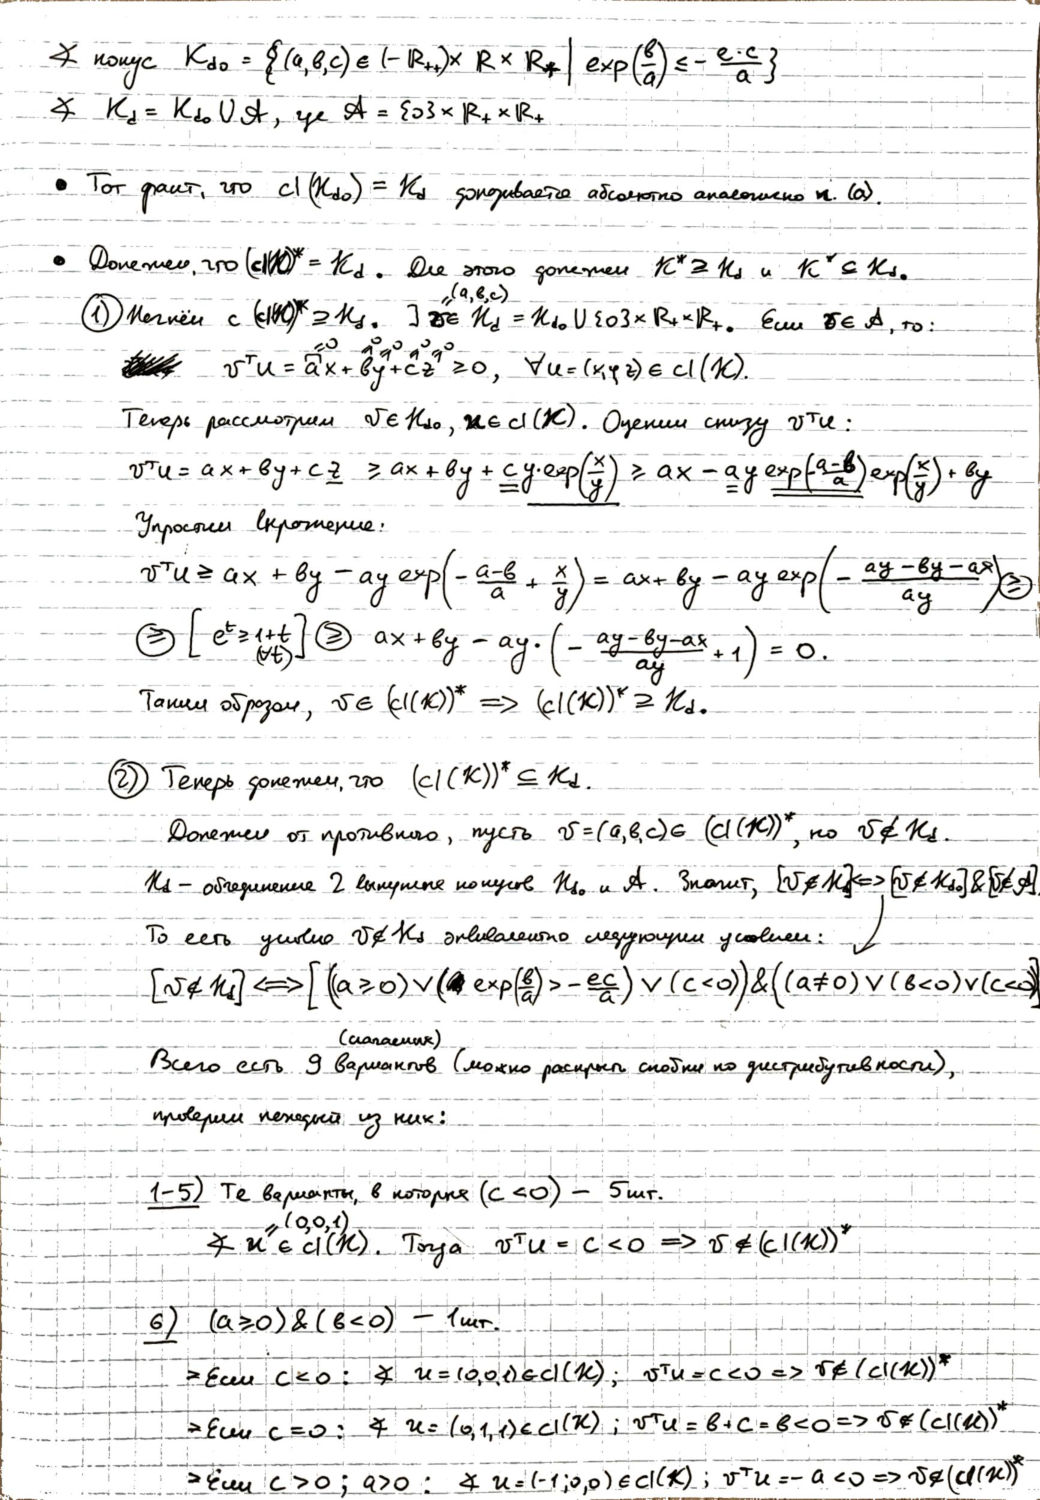
\includegraphics[width=0.82\linewidth]{figures/cone_1}
%	\end{figure}
%	\newpage
%	\begin{figure}[h!]
%		\centering
%		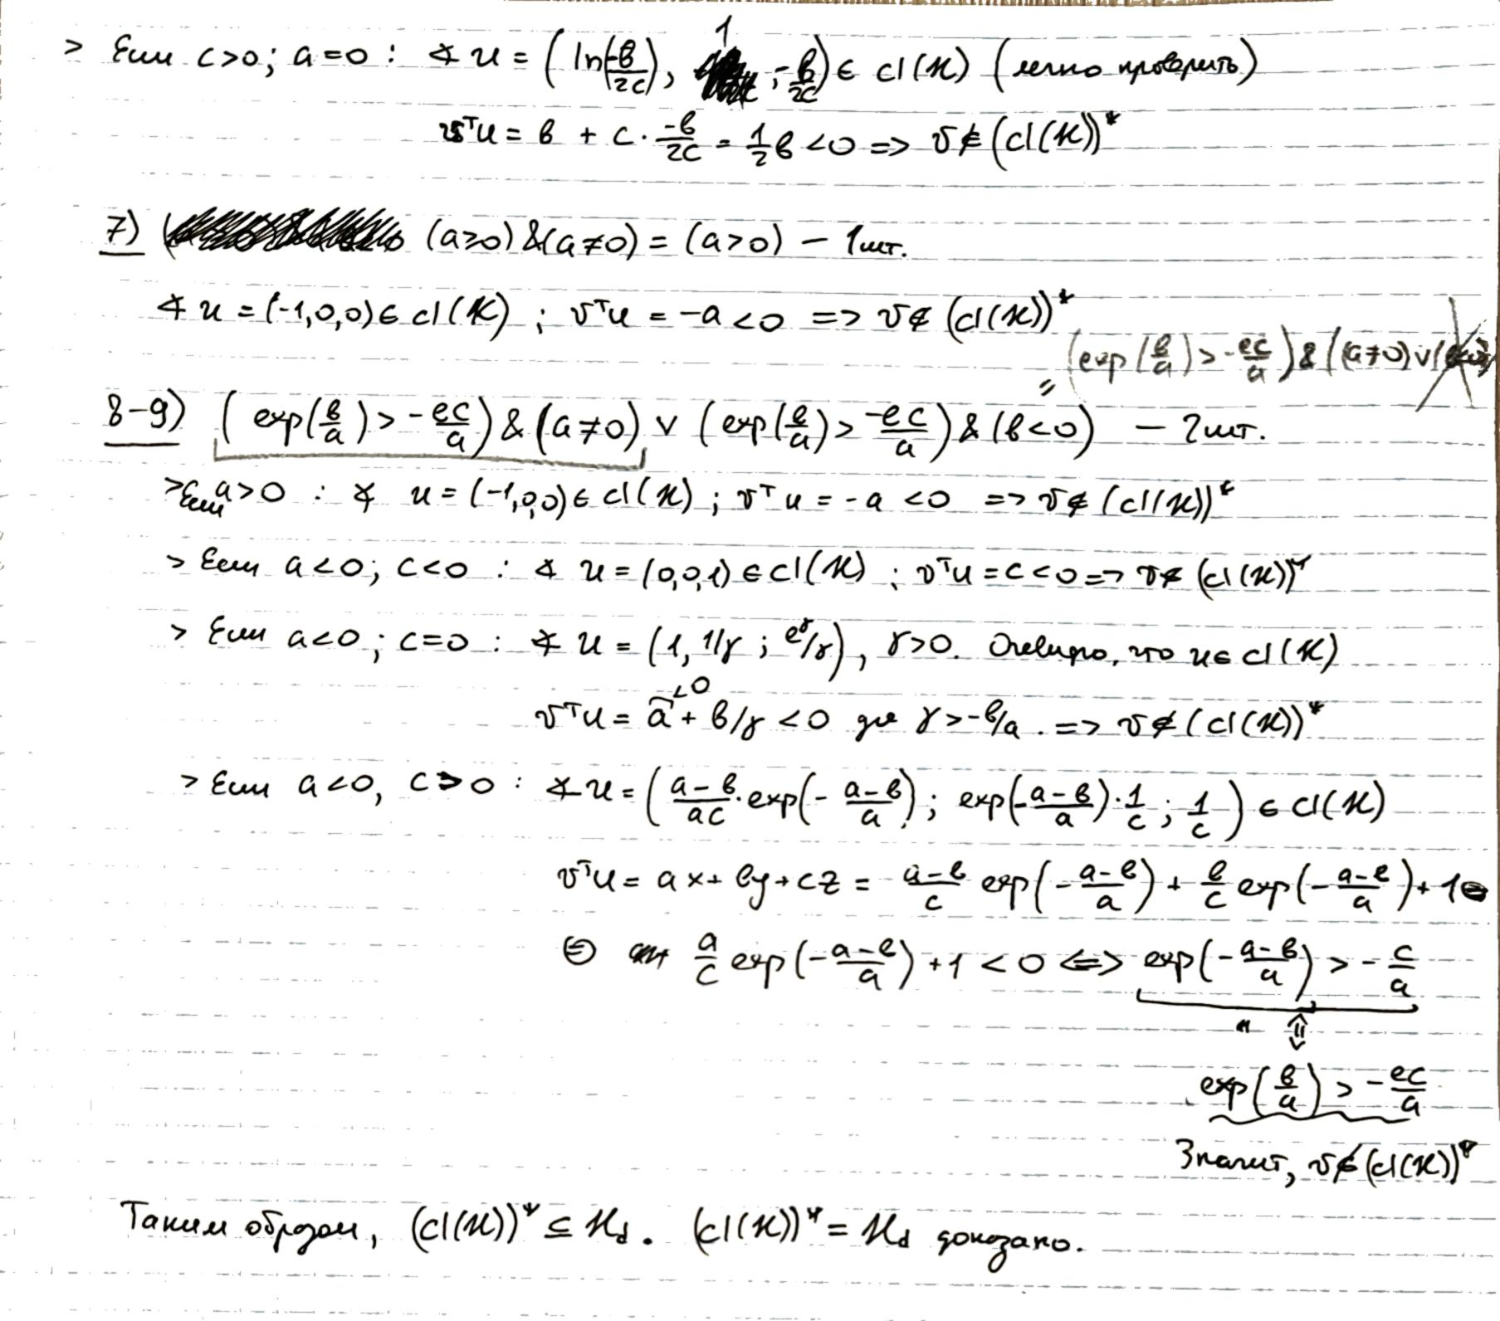
\includegraphics[width=0.82\linewidth]{figures/cone_2}
%	\end{figure}
	
	
\end{document}